%test git
%Template has reconstruct by xinhong landxh@gmail.com
%%%%%%%%%%%%%%%%%%%%%%%%%%%%%%%%%%%%%%%%%
% The Legrand Orange Book
% LaTeX Template
% Version 1.3 (21/8/13)
%
% This template has been downloaded from:
% http://www.LaTeXTemplates.com
%
% Original author:
% Mathias Legrand (legrand.mathias@gmail.com)
%
% License:
% CC BY-NC-SA 3.0 (http://creativecommons.org/licenses/by-nc-sa/3.0/)
%
% Compiling this template:
% This template uses biber for its bibliography and makeindex for its index.
% When you first open the template, compile it from the command line with the 
% commands below to make sure your LaTeX distribution is configured correctly:
%
% 1) pdflatex main
% 2) makeindex main.idx -s StyleInd.ist
% 3) biber main
% 4) pdflatex main x 2
%
% After this, when you wish to update the bibliography/index use the appropriate
% command above and make sure to compile with pdflatex several times 
% afterwards to propagate your changes to the document.
%
% This template also uses a number of packages which may need to be
% updated to the newest versions for the template to compile. It is strongly
% recommended you update your LaTeX distribution if you have any
% compilation errors.
%
% Important note:
% Chapter heading images should have a 2:1 width:height ratio,
% e.g. 920px width and 460px height.
%
%%%%%%%%%%%%%%%%%%%%%%%%%%%%%%%%%%%%%%%%%

%----------------------------------------------------------------------------------------
%	PACKAGES AND OTHER DOCUMENT CONFIGURATIONS
%----------------------------------------------------------------------------------------

\documentclass[11pt,fleqn]{book} % Default font size and left-justified equations

\usepackage[top=3cm,bottom=3cm,left=3.2cm,right=3.2cm,headsep=10pt,a4paper]{geometry} % Page margins

\usepackage{xcolor} % Required for specifying colors by name
\definecolor{ocre}{RGB}{120,190,255} % Define the orange color used for highlighting throughout the book

% Font Settings
\usepackage{avant} % Use the Avantgarde font for headings
%\usepackage{times} % Use the Times font for headings
\usepackage{mathptmx} % Use the Adobe Times Roman as the default text font together with math symbols from the Sym­bol, Chancery and Com­puter Modern fonts

\usepackage{microtype} % Slightly tweak font spacing for aesthetics
\usepackage[utf8]{inputenc} % Required for including letters with accents
\usepackage[T1]{fontenc} % Use 8-bit encoding that has 256 glyphs

% Bibliography
\usepackage[style=alphabetic,sorting=nyt,sortcites=true,autopunct=true,babel=hyphen,hyperref=true,abbreviate=false,backref=true,backend=biber]{biblatex}
\addbibresource{bibliography.bib} % BibTeX bibliography file
\defbibheading{bibempty}{}

% Index
\usepackage{calc} % For simpler calculation - used for spacing the index letter headings correctly

% read code file
\usepackage{ listings }

%----------------------------------------------------------------------------------------

%----------------------------------------------------------------------------------------
%	VARIOUS REQUIRED PACKAGES
%----------------------------------------------------------------------------------------

\usepackage{titlesec} % Allows customization of titles

\usepackage{graphicx} % Required for including pictures
\graphicspath{{Pictures/}} % Specifies the directory where pictures are stored

\usepackage{lipsum} % Inserts dummy text

\usepackage{tikz} % Required for drawing custom shapes

\usepackage[english]{babel} % English language/hyphenation

\usepackage{enumitem} % Customize lists
\setlist{nolistsep} % Reduce spacing between bullet points and numbered lists

\usepackage{booktabs} % Required for nicer horizontal rules in tables

\usepackage{eso-pic} % Required for specifying an image background in the title page

%----------------------------------------------------------------------------------------
%	MAIN TABLE OF CONTENTS
%----------------------------------------------------------------------------------------

\usepackage{titletoc} % Required for manipulating the table of contents

\contentsmargin{0cm} % Removes the default margin
% Chapter text styling
\titlecontents{chapter}[1.25cm] % Indentation
{\addvspace{15pt}\large\sffamily\bfseries} % Spacing and font options for chapters
{\color{ocre!60}\contentslabel[\Large\thecontentslabel]{1.25cm}\color{ocre}} % Chapter number
{}  
{\color{ocre!60}\normalsize\sffamily\bfseries\;\titlerule*[.5pc]{.}\;\thecontentspage} % Page number
% Section text styling
\titlecontents{section}[1.25cm] % Indentation
{\addvspace{5pt}\sffamily\bfseries} % Spacing and font options for sections
{\contentslabel[\thecontentslabel]{1.25cm}} % Section number
{}
{\sffamily\hfill\color{black}\thecontentspage} % Page number
[]
% Subsection text styling
\titlecontents{subsection}[1.25cm] % Indentation
{\addvspace{1pt}\sffamily\small} % Spacing and font options for subsections
{\contentslabel[\thecontentslabel]{1.25cm}} % Subsection number
{}
{\sffamily\;\titlerule*[.5pc]{.}\;\thecontentspage} % Page number
[] 

%----------------------------------------------------------------------------------------
%	MINI TABLE OF CONTENTS IN CHAPTER HEADS
%----------------------------------------------------------------------------------------

% Section text styling
\titlecontents{lsection}[0em] % Indendating
{\footnotesize\sffamily} % Font settings
{}
{}
{}

% Subsection text styling
\titlecontents{lsubsection}[.5em] % Indentation
{\normalfont\footnotesize\sffamily} % Font settings
{}
{}
{}
 
%----------------------------------------------------------------------------------------
%	PAGE HEADERS
%----------------------------------------------------------------------------------------

\usepackage{fancyhdr} % Required for header and footer configuration

\pagestyle{fancy}
\renewcommand{\chaptermark}[1]{\markboth{\sffamily\normalsize\bfseries #1}{}} % Chapter text font settings
\renewcommand{\sectionmark}[1]{\markright{\sffamily\normalsize\thesection\hspace{5pt}#1}{}} % Section text font settings
\fancyhf{} \fancyhead[LE,RO]{\sffamily\normalsize\thepage} % Font setting for the page number in the header
\fancyhead[LO]{\rightmark} % Print the nearest section name on the left side of odd pages
\fancyhead[RE]{\leftmark} % Print the current chapter name on the right side of even pages
\renewcommand{\headrulewidth}{0.5pt} % Width of the rule under the header
\addtolength{\headheight}{2.5pt} % Increase the spacing around the header slightly
\renewcommand{\footrulewidth}{0pt} % Removes the rule in the footer
\fancypagestyle{plain}{\fancyhead{}\renewcommand{\headrulewidth}{0pt}} % Style for when a plain pagestyle is specified

% Removes the header from odd empty pages at the end of chapters
\makeatletter
\renewcommand{\cleardoublepage}{
\clearpage\ifodd\c@page\else
\hbox{}
\vspace*{\fill}
\thispagestyle{empty}
\newpage
\fi}

%----------------------------------------------------------------------------------------
%	THEOREM STYLES
%----------------------------------------------------------------------------------------

\usepackage{amsmath,amsfonts,amssymb,amsthm} % For including math equations, theorems, symbols, etc

\newcommand{\intoo}[2]{\mathopen{]}#1\,;#2\mathclose{[}}
\newcommand{\ud}{\mathop{\mathrm{{}d}}\mathopen{}}
\newcommand{\intff}[2]{\mathopen{[}#1\,;#2\mathclose{]}}
\newtheorem{notation}{Notation}[chapter]

%%%%%%%%%%%%%%%%%%%%%%%%%%%%%%%%%%%%%%%%%%%%%%%%%%%%%%%%%%%%%%%%%%%%%%%%%%%
%%%%%%%%%%%%%%%%%%%% dedicated to boxed/framed environements %%%%%%%%%%%%%%
%%%%%%%%%%%%%%%%%%%%%%%%%%%%%%%%%%%%%%%%%%%%%%%%%%%%%%%%%%%%%%%%%%%%%%%%%%%
\newtheoremstyle{ocrenumbox}% % Theorem style name
{0pt}% Space above
{0pt}% Space below
{\normalfont}% % Body font
{}% Indent amount
{\small\bf\sffamily\color{ocre}}% % Theorem head font
{\;}% Punctuation after theorem head
{0.25em}% Space after theorem head
{\small\sffamily\color{ocre}\thmname{#1}\nobreakspace\thmnumber{\@ifnotempty{#1}{}\@upn{#2}}% Theorem text (e.g. Theorem 2.1)
\thmnote{\nobreakspace\the\thm@notefont\sffamily\bfseries\color{black}---\nobreakspace#3.}} % Optional theorem note
\renewcommand{\qedsymbol}{$\blacksquare$}% Optional qed square

\newtheoremstyle{blacknumex}% Theorem style name
{5pt}% Space above
{5pt}% Space below
{\normalfont}% Body font
{} % Indent amount
{\small\bf\sffamily}% Theorem head font
{\;}% Punctuation after theorem head
{0.25em}% Space after theorem head
{\small\sffamily{\tiny\ensuremath{\blacksquare}}\nobreakspace\thmname{#1}\nobreakspace\thmnumber{\@ifnotempty{#1}{}\@upn{#2}}% Theorem text (e.g. Theorem 2.1)
\thmnote{\nobreakspace\the\thm@notefont\sffamily\bfseries---\nobreakspace#3.}}% Optional theorem note

\newtheoremstyle{blacknumbox} % Theorem style name
{0pt}% Space above
{0pt}% Space below
{\normalfont}% Body font
{}% Indent amount
{\small\bf\sffamily}% Theorem head font
{\;}% Punctuation after theorem head
{0.25em}% Space after theorem head
{\small\sffamily\thmname{#1}\nobreakspace\thmnumber{\@ifnotempty{#1}{}\@upn{#2}}% Theorem text (e.g. Theorem 2.1)
\thmnote{\nobreakspace\the\thm@notefont\sffamily\bfseries---\nobreakspace#3.}}% Optional theorem note

%%%%%%%%%%%%%%%%%%%%%%%%%%%%%%%%%%%%%%%%%%%%%%%%%%%%%%%%%%%%%%%%%%%%%%%%%%%
%%%%%%%%%%%%% dedicated to non-boxed/non-framed environements %%%%%%%%%%%%%
%%%%%%%%%%%%%%%%%%%%%%%%%%%%%%%%%%%%%%%%%%%%%%%%%%%%%%%%%%%%%%%%%%%%%%%%%%%
\newtheoremstyle{ocrenum}% % Theorem style name
{5pt}% Space above
{5pt}% Space below
{\normalfont}% % Body font
{}% Indent amount
{\small\bf\sffamily\color{ocre}}% % Theorem head font
{\;}% Punctuation after theorem head
{0.25em}% Space after theorem head
{\small\sffamily\color{ocre}\thmname{#1}\nobreakspace\thmnumber{\@ifnotempty{#1}{}\@upn{#2}}% Theorem text (e.g. Theorem 2.1)
\thmnote{\nobreakspace\the\thm@notefont\sffamily\bfseries\color{black}---\nobreakspace#3.}} % Optional theorem note
\renewcommand{\qedsymbol}{$\blacksquare$}% Optional qed square
\makeatother

% Defines the theorem text style for each type of theorem to one of the three styles above
\newcounter{dummy} 
\numberwithin{dummy}{section}
\theoremstyle{ocrenumbox}
\newtheorem{theoremeT}[dummy]{Theorem}
\newtheorem{problem}{Problem}[chapter]
\newtheorem{exerciseT}{Exercise}[chapter]
\theoremstyle{blacknumex}
\newtheorem{exampleT}{Example}[chapter]
\theoremstyle{blacknumbox}
\newtheorem{vocabulary}{Vocabulary}[chapter]
\newtheorem{definitionT}{Definition}[section]
\newtheorem{corollaryT}[dummy]{Corollary}
\theoremstyle{ocrenum}
\newtheorem{proposition}[dummy]{Proposition}

%----------------------------------------------------------------------------------------
%	DEFINITION OF Code BLOCK
%----------------------------------------------------------------------------------------

\lstdefinestyle{custom}{
  belowcaptionskip=1\baselineskip,
  breaklines=true,
  frame=L,
  xleftmargin=\parindent,
  showstringspaces=false,
  basicstyle=\scriptsize\ttfamily,
  keywordstyle=\bfseries\color{green!40!black},
  commentstyle=\itshape\color{purple!40!black},
  identifierstyle=\color{brown},
  stringstyle=\color{rbrown},
}

\lstdefinestyle{customc}{
  belowcaptionskip=1\baselineskip,
  breaklines=true,
  frame=L,
  xleftmargin=\parindent,
  language=C,
  showstringspaces=false,
  basicstyle=\scriptsize\ttfamily,
  keywordstyle=\bfseries\color{green!40!black},
  commentstyle=\itshape\color{purple!40!black},
  identifierstyle=\color{blue},
  stringstyle=\color{orange},
}

\lstdefinestyle{customasm}{
  belowcaptionskip=1\baselineskip,
  frame=L,
  xleftmargin=\parindent,
  language=[x86masm]Assembler,
  basicstyle=\scriptsize\ttfamily,
  commentstyle=\itshape\color{purple!40!black},
}

\lstset{escapechar=@,style=custom}

%----------------------------------------------------------------------------------------
%	DEFINITION OF COLORED BOXES
%----------------------------------------------------------------------------------------

\RequirePackage[framemethod=default]{mdframed} % Required for creating the theorem, definition, exercise and corollary boxes

% Theorem box
\newmdenv[skipabove=7pt,
skipbelow=7pt,
backgroundcolor=black!5,
linecolor=ocre,
innerleftmargin=5pt,
innerrightmargin=5pt,
innertopmargin=5pt,
leftmargin=0cm,
rightmargin=0cm,
innerbottommargin=5pt]{tBox}

% Exercise box	  
\newmdenv[skipabove=7pt,
skipbelow=7pt,
rightline=false,
leftline=true,
topline=false,
bottomline=false,
backgroundcolor=ocre!10,
linecolor=ocre,
innerleftmargin=5pt,
innerrightmargin=5pt,
innertopmargin=5pt,
innerbottommargin=5pt,
leftmargin=0cm,
rightmargin=0cm,
linewidth=4pt]{eBox}	

% Definition box
\newmdenv[skipabove=7pt,
skipbelow=7pt,
rightline=false,
leftline=true,
topline=false,
bottomline=false,
linecolor=ocre,
innerleftmargin=5pt,
innerrightmargin=5pt,
innertopmargin=0pt,
leftmargin=0cm,
rightmargin=0cm,
linewidth=4pt,
innerbottommargin=0pt]{dBox}	

% Corollary box
\newmdenv[skipabove=7pt,
skipbelow=7pt,
rightline=false,
leftline=true,
topline=false,
bottomline=false,
linecolor=gray,
backgroundcolor=black!5,
innerleftmargin=5pt,
innerrightmargin=5pt,
innertopmargin=5pt,
leftmargin=0cm,
rightmargin=0cm,
linewidth=4pt,
innerbottommargin=5pt]{cBox}				  
		  

% Creates an environment for each type of theorem and assigns it a theorem text style from the "Theorem Styles" section above and a colored box from above
\newenvironment{theorem}{\begin{tBox}\begin{theoremeT}}{\end{theoremeT}\end{tBox}}
\newenvironment{exercise}{\begin{eBox}\begin{exerciseT}}{\hfill{\color{ocre}\tiny\ensuremath{\blacksquare}}\end{exerciseT}\end{eBox}}				  
\newenvironment{definition}{\begin{dBox}\begin{definitionT}}{\end{definitionT}\end{dBox}}	
\newenvironment{example}{\begin{exampleT}}{\hfill{\tiny\ensuremath{\blacksquare}}\end{exampleT}}		
\newenvironment{corollary}{\begin{cBox}\begin{corollaryT}}{\end{corollaryT}\end{cBox}}	

%----------------------------------------------------------------------------------------
%	REMARK ENVIRONMENT
%----------------------------------------------------------------------------------------

\newenvironment{remark}{\par\vskip10pt\small % Vertical white space above the remark and smaller font size
\begin{list}{}{
\leftmargin=35pt % Indentation on the left
\rightmargin=25pt}\item\ignorespaces % Indentation on the right
\makebox[-2.5pt]{\begin{tikzpicture}[overlay]
\node[draw=ocre!60,line width=1pt,circle,fill=ocre!25,font=\sffamily\bfseries,inner sep=2pt,outer sep=0pt] at (-15pt,0pt){\textcolor{ocre}{R}};\end{tikzpicture}} % Orange R in a circle
\advance\baselineskip -1pt}{\end{list}\vskip5pt} % Tighter line spacing and white space after remark

%----------------------------------------------------------------------------------------
%	SECTION NUMBERING IN THE MARGIN
%----------------------------------------------------------------------------------------

\makeatletter
\renewcommand{\@seccntformat}[1]{\llap{\textcolor{ocre}{\csname the#1\endcsname}\hspace{1em}}}                    
\renewcommand{\section}{\@startsection{section}{1}{\z@}
{-4ex \@plus -1ex \@minus -.4ex}
{1ex \@plus.2ex }
{\normalfont\large\sffamily\bfseries}}
\renewcommand{\subsection}{\@startsection {subsection}{2}{\z@}
{-3ex \@plus -0.1ex \@minus -.4ex}
{0.5ex \@plus.2ex }
{\normalfont\sffamily\bfseries}}
\renewcommand{\subsubsection}{\@startsection {subsubsection}{3}{\z@}
{-2ex \@plus -0.1ex \@minus -.2ex}
{0.2ex \@plus.2ex }
{\normalfont\small\sffamily\bfseries}}                        
\renewcommand\paragraph{\@startsection{paragraph}{4}{\z@}
{-2ex \@plus-.2ex \@minus .2ex}
{0.1ex}
{\normalfont\small\sffamily\bfseries}}

%----------------------------------------------------------------------------------------
%	CHAPTER HEADINGS
%----------------------------------------------------------------------------------------

\newcommand{\thechapterimage}{}
\newcommand{\chapterimage}[1]{\renewcommand{\thechapterimage}{#1}}
\def\thechapter{\arabic{chapter}}
\def\@makechapterhead#1{
\thispagestyle{empty}
{\centering \normalfont\sffamily
\ifnum \c@secnumdepth >\m@ne
\if@mainmatter
\startcontents
\begin{tikzpicture}[remember picture,overlay]
\node at (current page.north west)
{\begin{tikzpicture}[remember picture,overlay]

\node[anchor=north west,inner sep=0pt] at (0,0) {\includegraphics[width=\paperwidth]{\thechapterimage}};

%Commenting the 3 lines below removes the small contents box in the chapter heading
\draw[fill=white,opacity=.6] (1cm,0) rectangle (8cm,-7cm);
\node[anchor=north west] at (1cm,.25cm) {\parbox[t][8cm][t]{6.5cm}{\huge\bfseries\flushleft \printcontents{l}{1}{\setcounter{tocdepth}{2}}}};

\draw[anchor=west] (5cm,-9cm) node [rounded corners=25pt,fill=white,fill opacity=.6,text opacity=1,draw=ocre,draw opacity=1,line width=2pt,inner sep=15pt]{\huge\sffamily\bfseries\textcolor{black}{\thechapter\ ---\ #1\vphantom{plPQq}\makebox[22cm]{}}};
\end{tikzpicture}};
\end{tikzpicture}}\par\vspace*{230\p@}
\fi
\fi
}
\def\@makeschapterhead#1{
\thispagestyle{empty}
{\centering \normalfont\sffamily
\ifnum \c@secnumdepth >\m@ne
\if@mainmatter
\startcontents
\begin{tikzpicture}[remember picture,overlay]
\node at (current page.north west)
{\begin{tikzpicture}[remember picture,overlay]
\node[anchor=north west] at (-4pt,4pt) {\includegraphics[width=\paperwidth]{\thechapterimage}};
\draw[anchor=west] (5cm,-9cm) node [rounded corners=25pt,fill=white,opacity=.7,inner sep=15.5pt]{\huge\sffamily\bfseries\textcolor{black}{\vphantom{plPQq}\makebox[22cm]{}}};
\draw[anchor=west] (5cm,-9cm) node [rounded corners=25pt,draw=ocre,line width=2pt,inner sep=15pt]{\huge\sffamily\bfseries\textcolor{black}{#1\vphantom{plPQq}\makebox[22cm]{}}};
\end{tikzpicture}};
\end{tikzpicture}}\par\vspace*{230\p@}
\fi
\fi
}
\makeatother % Insert the commands.tex file which contains the majority of the structure behind the template

\begin{document}

%----------------------------------------------------------------------------------------
%	TITLE PAGE
%----------------------------------------------------------------------------------------

\begingroup
\thispagestyle{empty}
%\AddToShipoutPicture*{\put(6,5){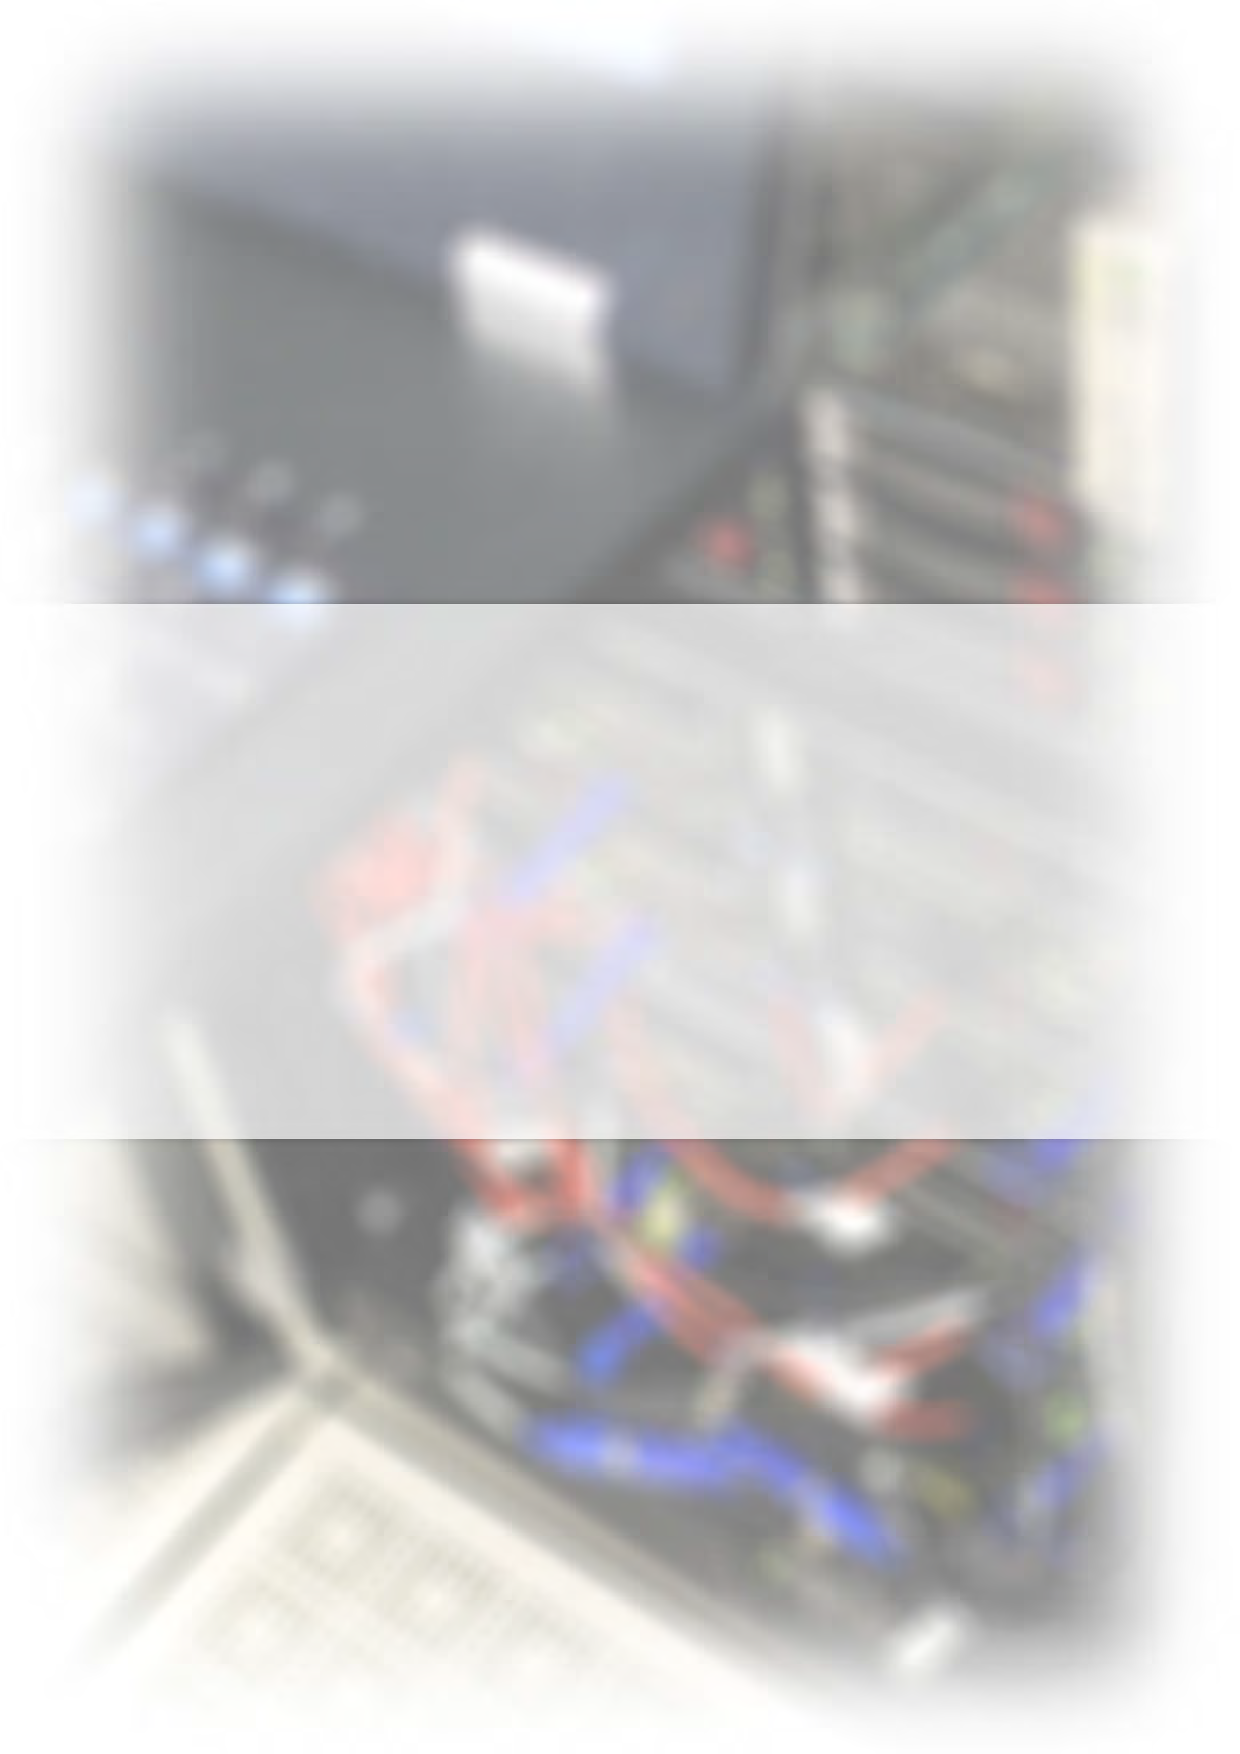
\includegraphics[scale=1]{background}}} % Image background
\centering
\vspace*{9cm}
\par\normalfont\fontsize{35}{35}\sffamily\selectfont
Combo Manual\par % Book title
\vspace*{1cm}
{\Large Kickstarter to Master}\par
{\tiny Things You May Want to Know}\par % 
\endgroup

%----------------------------------------------------------------------------------------
%	COPYRIGHT PAGE
%----------------------------------------------------------------------------------------

\newpage
~\vfill
\thispagestyle{empty}

\noindent Copyright \copyright\ 2014 Computational Biophysics and Materials Science Group\\ % Copyright notice

\noindent \textsc{Published}\\ % Publisher

\noindent \textsc{ourphysics.org}\\ % URL

\noindent This manual basicly list the problems you may encounter when you maintain the combo, or reinstall the combo.\\ % License information

\noindent \textit{V1.1.0, March 2014} % Printing/edition date

%----------------------------------------------------------------------------------------
%	TABLE OF CONTENTS
%----------------------------------------------------------------------------------------

\chapterimage{chapter_head_1.pdf} % Table of contents heading image

\pagestyle{empty} % No headers

\tableofcontents % Print the table of contents itself

\cleardoublepage % Forces the first chapter to start on an odd page so it's on the right

\pagestyle{fancy} % Print headers again

%----------------------------------------------------------------------------------------
%	CHAPTER 1
%----------------------------------------------------------------------------------------
\chapterimage{chapter_head_2.pdf} 
\chapter{Introduction}
\section{Terminology}\index{Terminology}

\section{Name}
\subsection{Hardware}
\begin{description}
\item[Frontend] a computer, also called "server node" to connect and control the computer nodes.
\item[Computer Node] a computer, connected and controlled by frontend, and can do process jobs.
\end{description}
\subsection{Non-Hardware}
\begin{description}
\item[Combo] Combo is a nick name of our cluster.
\item[Computer cluster] A computer cluster consists of a set of loosely connected or tightly connected computers that work together so that in many respects they can be viewed as a single system.\footnote{From WikiPedia - Item:Computer cluster, http://en.wikipedia.org/wiki/Cluster\_(computing), retrived on Mar 21, 2014}
\item[MPI] Message Passing Interface (MPI) is a standardized and portable message-passing system designed by a group of researchers from academia and industry to function on a wide variety of parallel computers. The standard defines the syntax and semantics of a core of library routines useful to a wide range of users writing portable message-passing programs in Fortran or the C programming language. There are several well-tested and efficient implementations of MPI, including some that are free or in the public domain. These fostered the development of a parallel software industry, and there encouraged development of portable and scalable large-scale parallel applications.\footnote{From WikiPedia - Item:Message Passing Interface, http://en.wikipedia.org/wiki/Message\_Passing\_Interface, retrived on Mar 21, 2014}
\item[Parallel computing] Parallel computing is a form of computation in which many calculations are carried out simultaneously, operating on the principle that large problems can often be divided into smaller ones, which are then solved concurrently ("in parallel"). There are several different forms of parallel computing: bit-level, instruction level, data, and task parallelism. Parallelism has been employed for many years, mainly in high-performance computing, but interest in it has grown lately due to the physical constraints preventing frequency scaling. As power consumption (and consequently heat generation) by computers has become a concern in recent years, parallel computing has become the dominant paradigm in computer architecture, mainly in the form of multi-core processors.\footnote{From WikiPedia - Item:Parallel computing, http://en.wikipedia.org/wiki/Parallel\_computing, retrived on Mar 21, 2014}
\item[Rocks] Rocks is an open-source Linux cluster distribution that enables end users to easily build computational clusters, grid endpoints and visualization tiled-display walls.\footnote{Rocks Official Website, http://www.rocksclusters.org/wordpress/?page\_id=57, retrived on Mar 21, 2014} Rocks was initially based on the Red Hat Linux distribution, however modern versions of Rocks were based on CentOS, with a modified Anaconda installer that simplifies mass installation onto many computers. \footnote{From WikiPedia - Item:Rocks Cluster Distribution, http://en.wikipedia.org/wiki/Rocks\_Cluster\_Distribution, retrived on Mar 21, 2014}
\end{description}

\section{Notation}
\subsection{Code}
In this manual, there are a lot of code example, to make it clear to distinguish code from others, some explaination are needed:
\paragraph{Command Line}
\begin{enumerate}
\item Each command will start with "{\tt \$}", the font is typewriter font, with various font sizes.
\item If a piece of command is too long to place in one line, a "{\tt \textbackslash}" is used to indicate ignoring a linebreak.
\item try not to directly copy from this manual and paste in terminal, for sometiomes "{\tt $\sim$}" and "{\tt \_}" may looks good in manual, but inappropriate in ternimal, pay attention when you paste a block of codes.
\end{enumerate}




\section{Hardware}\index{Hardware}

Introduction about hardware of combo.

\subsection{Processor}\index{Processor}

\begin{itemize}
\item $32$ CPUs for frontend
\item $16 \times 16$ CPUs for nodes
\item $16 \times 1$ GPUs for nodes
\end{itemize}

\subsection{Communication}\index{Communication}

\begin{itemize}
\item $1 \times HP 2910-48G Switch $
\item $1 \times Vo.. Switch $
\end{itemize}

%------------------------------------------------

\section{Structure}\index{Structure}

To quickly understand how the combo works, we can image there are a team of army consisting of 16 solders as well as a captain. 

%------------------------------------------------

\section{Software}\index{Software}

Here list the softwares installed on Combo.

\subsection{Operation System}\index{Operation System}

The operating system is Rocks\footnote{http://rocksclusters.org}, Currect version is ver.6.2.

\subsection{Compiler}\index{Compiler}

\begin{itemize}
\item GNU Compiler (gcc, g++, fortran, JAVA...)
\end{itemize}

\subsection{Development Tools}\index{Development Tools}

\begin{itemize}
\item NVIDIA CUDA Toolkit\footnote{https://developer.nvidia.com/cuda-toolkit}
\end{itemize}

%----------------------------------------------------------------------------------------
%	CHAPTER 2
%----------------------------------------------------------------------------------------
\chapterimage{chapter_head_2.pdf} % Chapter heading image
\chapter{Installation}\index{Installation}
To install the combo, basically, the following steps need to follow:

\begin{enumerate}
\item Install the Rocks in the frontend
\item Connect the computer nodes to frontend
\item Install the applications
\end{enumerate}

Then, the details are as followed:

\section{Installing Operating System}\index{Installing Operating System}

Installing operating system on frontend is as easy as you install Windows on your PC, once you know how to config right. \\
And what I am exactly doing here, is to let you know, how to do it right:
\begin{enumerate}
\item Download the .ISO and burn into the DVD
\item Put DVD into optical driver and follow the prompt to do one step after another.
\item done
\end{enumerate}

\subsection{Download .ISO file and Boot from DVD}
The file can be download from \url{http://www.rocksclusters.org/wordpress/?page_id=80 }, the architacture is x86\_64 and the jumpo DVD is preferred. 

\begin{remark}
The installation guide is availible on \url{http://www.rocksclusters.org/wordpress/?page_id=4}, to avoid iterance, only those with special attention are listed.
\end{remark}

\subsection{Selecting Rolls}
At beginning, you are required to select rolls to install. Of course, tick them all is a safe choice, anyway, I will list the rolls recommended to be installed on frontend:
\begin{remark}
\begin{description}
\item[Roll] In Rocks, a roll can be regarded as a package, The "Rolls" extend the system by integrating seamlessly and automatically into the management and packaging mechanisms used by base software, greatly simplifying installation and configuration of large numbers of computers.\footnote{Breaking News - Operating Systems \& Middleware: SDSC Enhances Rocks Cluster Management Toolkit, http://web.archive.org/web/20070927031015/http://www.gridtoday.com/04/0216/102698.html, retrived on Mar 19, 2014}.
\end{description}
\end{remark}
\begin{enumerate}
\item boot,
\item base, 
\item ganglia, 
\item HPC,
\item python, 
\item os,
\item kernel,
\end{enumerate}

\subsection{Network Settings}
In the this section, pay {\bf attention} to network configuration. If you have never plugged the wires, the default interface is:
\begin{itemize}
\item eth2: Private Network: 192.168.1.18: Netmask: 255.255.0.0
\item eth3: Public Network: 144.214.25.68: Netmask: 255.255.0.0
\begin{remark}
Do not choose {\it eth0} or {\it eth1}, or you will suffer a lot afterwards.
\end{remark}
\item Gateway: 144.214.2.254: DNS Server: 144.214.5.20
\begin{remark}
These settings are according to CityU CSC.
\end{remark}
\end{itemize}
Anyway, make sure every textbox is filled appropriately except longitude and latitude.

\subsection{Disk Partition}
To better manage our cluster, manual disk partition is required. If it is a reinstallation, delete all the existing partition. Then simply press "add". /dev/sdaN (where N is a number starts from 1) will be created automatically. Maximum number for N is 5, after 5 it will create new devices automatically. However ext4 might have the problem of a maximum volume of 16T, therefore /data and /data2 should be specially created using logical volumes. 
\paragraph{Partition Setting}
\begin{tabular}{ | r | c | c | c |}
	\hline
		File System & Mounted on & Size (MB) & Format $?$ \\ \hline
		 & / & 20000 & yes \\ \hline
		 & /boot & 500 & yes \\ \hline
		 & /var & 5000 & yes \\ \hline
		 & swap & 10000 & yes \\ \hline
		 & /export & max & yes \\ \hline
		/dev/mapper/vg\_combo\_LogVol00 & /data & 11T & no \\ \hline
		/dev/mapper/vg\_combo\_LogVol01 & /data2 & 9T & no \\
	\hline
\end{tabular}

\section{Before Connecting Conputer Nodes*}
This part is very special, because the {\bf torque} is preferred to be installed before connecting computer nodes. The reason is what we use is {\bf Torque Roll}, it will automatically identify nodes only when nodes are added after torque installed. 

\subsection{TORQUE}
Torque is not packaged in rocks DVD, we need to download torque\footnote{Torque+Maui job queueing system, packaged by HPC Group at University of Tromso, Norway} from \url{ftp://ftp.uit.no/pub/linux/rocks/torque-roll/}.
\begin{enumerate}
\item under {\tt /export/rocks/install }(ensure you are there), run \\ {\tt \$ rocks add roll /root/Desktop/torque-6.0.0-1.x86\_64.disk1.iso } (differ if the ISO file differs),
\item {\tt \$ rocks enable roll torque },
\item {\tt \$ rocks create distro }(make sure you are really in {\tt /export/rocks/install}, for this step is to create a Rocks distribution, which is used to install Rocks nodes with torque.)
\item {\tt \$ rocks run roll torque | sh }(run the torque roll),
\item {\tt \$ reboot }(after reboot, you can use {\tt \$ pbsnodes -a} to see whether it is running or not)
\end{enumerate}
\begin{remark}
I have to complain about torque here. The version Rocks Official Website\footnote{http://www.rocksclusters.org/} recommend torque package from {\it HPC Group at University of Tromso, Norway}, which is version 6.0.0. I cannot find any documentation or tutorial of this version. Oh that is terribly annoying. If you did not pay attention to the small-size introduction about Rocks, and Google "torque", you will find another torque...
\end{remark}

We are about to connect computer nodes, if you do not want to create partitions one by one, here's a trick! You might create a XML file for nodes to read when creating their partitions:
\begin{itemize}
\item {\tt \$ cd /export/rocks/install/site-profiles/6.2/nodes/}
\item {\tt \$ cp skeleton.xml replace-partition.xml}
\item {\tt \$ vi replace-partition.xml}
\end{itemize}
Then insert the following lines in-between <pre> and </pre>:
\begin{lstlisting}[basicstyle=\ttfamily\scriptsize,columns=fullflexible]
<pre>
echo "clearpart --all --initlabel --drivers=sda
part / --size 100000 --ondisk sda
part swap --size 80000 --ondisk sda
part /mydata --size 1 --grow --ondisk sda" > /tmp/user_partition_info
</pre>
\end{lstlisting}
Remember to execute 
\begin{itemize}
\item {\tt \$ rocks create distro}
\end{itemize}
in order to make it work.

\section{Connecting Computer Nodes}
Just mentioned before, frontend is {\it "Caption"} and we need to establish connections among {\it "Caption"} and {\it "Solders"}.
\begin{enumerate}
\item Ensure you have installed Torque roll and rebooted,
\item Cut off Internet, Shutdown all the nodes by your hands,
\begin{remark}
The reason for cutting off internet is that if someone knock on Combo during insert-ether, Combo will recognise it as a node which is obviously not preferable. 
\end{remark}
\item Open Terminal, run {\tt \$ insert-ethers}, choose {\bf Compute} as type,
\item boot each node one by one, (take your time, maybe switch on one every 1 min), choose "Network Booting" when prompted,
\item partition nodes according to: \\
\begin{tabular}{ r | c | c | l }
	\hline
		File System & Mounted on & Size & Format ? \\ \hline
		/dev/sda2 & / & 100000 & yes \\ \hline
		/dev/sda1 & swap & 80000 & yes \\ \hline
		/dev/sdb & /mydata & whatever & yes \\
	\hline
\end{tabular}
\end{enumerate}

\section{Installing Applications}
The most challenging mission just starts. In this section, we need to install several applications. We will deal with them one by one.

\subsection{NVIDIA CUDA Toolkit}
Install CUDA is relatively easy, first install NVIDIA driver, then CUDA Toolkit. CUDA Toolkit could be download from \url{https://developer.nvidia.com/cuda-downloads}, the installation guide on official website(url{http://docs.nvidia.com/cuda/cuda-getting-started-guide-for-linux/index.html}), here only list some interesting points: (Applied to NVIDIA CUDA Getting Started Guide for Linux, DU-05347-001\_v5.5, July 19, 2013)
\begin{enumerate}
\item {\tt \$ sh cuda-linux64-rel-5.5.22-16488124.run -extract=/share/apps/cuda-install }
\item {\tt \$ sudo sh cuda-linux64-rel-5.5.22-16488124.run -prefix=/share/apps/cuda }
\item add folowing code to $\sim$/.bashrc:
\begin{lstlisting}[basicstyle=\ttfamily\scriptsize,columns=fullflexible]
# Setting for CUDA
export PATH=/share/apps/cuda/bin:$PATH
export LD_LIBRARY_PATH=/share/apps/cuda/lib64:$LD_LIBRARY_PATH
export LD_LIBRARY_PATH=/share/apps/cuda/lib:$LD_LIBRARY_PATH
\end{lstlisting}
\begin{remark}
Here is a trick to quickly sync the .bashrc to all node, use the code in frontend:
\lstinputlisting[basicstyle=\ttfamily\scriptsize,columns=fullflexible,breaklines=true,]{./code/sync_bashrc}
\end{remark}
\item {\tt \$ source $\sim$/.bashrc } to update environment variables, and do this to each node.
\item Next, you need to install NVIDIA driver to each node. on each node, run \\ 
{\tt \$ /share/apps/cuda/NVIDIA-Linux-x86\_64-319.37.run } \\
on each node, follow prompt.
\end{enumerate}
\begin{itemize}
\item To test whether CUDA is set up, do the following test steps(I found the test method on the official guide is somehow incorrect, here is the apprepriate method):
\begin{enumerate}
\item run {\tt \$ cuda-install-samples-5.5.sh $\sim$} in CUDA installation directory,
\item {\tt \$ cd $\sim$/NVIDIA\_CUDA-5.5\_Samples/1\_Utilities/deviceQuery/},
\item {\tt \$ make},
\item {\tt \$ ./deviceQuery},
\end{enumerate}
You will see "{\tt Result = PASS}" at the end of terminal window if CUDA is set up right.
\end{itemize}
\subsection{Intel Parallel Studio}
Intel Parallel Studio is not a free software, to use it legally and without cost, we need to register for non-commercial version(\url{http://software.intel.com/en-us/non-commercial-software-development}).
\begin{itemize}
\item download the {\bf parallel\_studio\_xe\_2013\_sp1\_update1.tgz}, place it somewhere, untar it using {\tt \$ tar -xzvf parallel\_studio\_xe\_2013\_sp1\_update1.tgz}.
\item You can either choose to run install\_GUI.sh or install.sh program under uncompressed directory, follow prompt.
\item When there is {\bf Custom} or {\bf Advanced} option, choose them.
\item When prompted to define the installation location, use {\tt /share/apps/} as target directory.
\item x86 option can be ticked can also be unticked. Ignore the warning at the end if you did not tick to install x86 compilers. 
\end{itemize}
\begin{remark}
Remember to put the following codes into $\sim$/.bashrc:
\begin{lstlisting}[basicstyle=\ttfamily\scriptsize,columns=fullflexible]
#for Interl mkl
source /share/apps/intel/mkl/bin/mklvars.sh intel64
\end{lstlisting}
\end{remark}
\subsection{OpenMPI}
I followed this blog\footnote{Shane Tarleton, Install OpenMPI with GNU Compilers, 
http://www.shanetarleton.com/install-openmpi-with-gnu-compilers} to install OpenMPI. Maybe someday this blog disappears, then you cannot find it, in case, I will lead you through it. 
\begin{enumerate}
\item I found till now, we do not have {\bf g++} compiler installed, use {\tt \$ yum install gcc-c++} to install {\bf g++} compiler first.
\item copy the following code to {\bf $\sim$/.bashrc} if they are not there:
\lstinputlisting[basicstyle=\ttfamily\scriptsize,columns=fullflexible]{./code/bashrc_before_openmpi}
\item run {\tt \$ source $\sim$/.bashrc} to make bashrc file work.
\item download OpenMPI from \url{http://www.open-mpi.org/}, and place into {\bf /share/apps/}
\item then create 2 folders in {\bf /share/apps/}:
\begin{lstlisting}[basicstyle=\ttfamily\scriptsize,columns=fullflexible]
cd /share/apps
mkdir openmpi-install
mkdir openmpi-1.6.5
\end{lstlisting}
\item run {\tt \$ tar -C openmpi-install -xf openmpi-1.6.5.tar.gz} to uncompress it into {\bf openmpi-install folder}, then {\tt cd} into the folder.
\item run {\tt \$ ./configure --prefix=/share/apps/openmpi-1.6.5} to do install configure, 
\item then run {\tt \$ make all install} to install it.
\item add folowing code to {\bf $\sim$/.bashrc}:
\begin{lstlisting}[basicstyle=\ttfamily\scriptsize,columns=fullflexible]
# Settings for OpenMPI
export PATH=/share/apps/openmpi-1.6.5/bin:$PATH
export INCLUDE=/share/apps/openmpi-1.6.5/include:$INCLUDE
export LD_LIBRARY_PATH=/share/apps/openmpi-1.6.5/lib:$LD_LIBRARY_PATH
\end{lstlisting}
also, run {\tt \$ source $\sim$/.bashrc} to make it work.
and till now, the {\bf $\sim$/.bashrc} file should look like this:
\lstinputlisting[basicstyle=\ttfamily\scriptsize,columns=fullflexible]{./code/bashrc_after_openmpi}
\end{enumerate}
\subsection{NAMD}
(Added on 12 July 2015 when we are doing the reinstallation of Combo after an unknown attack causing the whole thing to crash) \\
Generally I followed the release note of NAMD (Here\footnote{http://www.ks.uiuc.edu/Research/namd/2.10/notes.html} for NAMD 2.10) and I do recommend all of you to do so. Do not bother to understand every word of it for the first glance, but do bear in mind that they are one of the criteria for your understanding of UIUC softwares. In the following section, I would try to combine what they tell us about a MPI (probably with InfiniBand) plus CUDA version of NAMD 2.10 so you do not have to scroll up and down the page. 
\begin{itemize}
\item Firstly of cause, download the correct tar ball (2015/07/15: NAMD\_2.10\_Source.tar) and send it to Combo using your own method (e.g. FileZilla or scp).
\item tar xvf NAMD\_2.10\_Source.tar.gz
\begin{remark}
I am not sure why the release note suggests xzf options and also the file is end with gz extension while I can only untar the file using xf options showing that the file is NOT zipped. Anyway, it does not matter much. 
\end{remark}
\item cd NAMD\_2.10\_Source
\item tar xvf charm-6.6.1.tar
\item cd charm-6.6.1
\item env MPICXX=mpicxx ./build charm++ mpi-linux-x86\_64 --with-production
\begin{remark}
In fact you can simply type ./build to enter an interactive mode choosing compilation options one by one and I DO recommend you to try that. 
\end{remark}
\item cd mpi-linux-x86\_64/tests/charm++/megatest
\item make pgm
\item mpirun -n 4 ./pgm   (run as any other MPI program on your cluster)
\item cd ../../../../..   (go to the very original NAMD\_2.10\_Source directory)
\begin{remark}
I do recommend you to copy the following lines into a bash script instead of copying them to the console one by one.
\end{remark}
\item wget http://www.ks.uiuc.edu/Research/namd/libraries/fftw-linux-x86\_64.tar.gz 
\item tar xzf fftw-linux-x86\_64.tar.gz mv linux-x86\_64 fftw 
\item wget http://www.ks.uiuc.edu/Research/namd/libraries/tcl8.5.9-linux-x86\_64.tar.gz 
\item wget http://www.ks.uiuc.edu/Research/namd/libraries/tcl8.5.9-linux-x86\_64-threaded.tar.gz 
\item tar xzf tcl8.5.9-linux-x86\_64.tar.gz 
\item tar xzf tcl8.5.9-linux-x86\_64-threaded.tar.gz 
\item mv tcl8.5.9-linux-x86\_64 tcl 
\item mv tcl8.5.9-linux-x86\_64-threaded tcl-threaded
\item ./config Linux-x86\_64-g++ --charm-arch mpi-linux-x86\_64 --with-cuda --cuda-prefix /share/apps/cuda
\begin{remark}
What follows the --charm-arch is the name of your charm build directory.
\end{remark}
\item cd Linux-x86\_64-g++
\item gmake -j32
\item ./namd2 src/alanin
\item mpirun -n 4 ./namd2 src/alanin
\end{itemize}
\subsection{FFTW and GROMACS}
Installing FFTW and GROMACS should be difficult if you have not ever experienced. Don't worry, our Kevin has worked out the right way to install it and you, just need to do copy and paste work. :-)
\begin{remark}
I still want to make sure again you have got {\bf g++} installed. if not, run {\tt \$ yum install gcc-c++}(if installed, you can still run it to make sure).
\end{remark}
\subsubsection{FFTW}
\begin{enumerate}
\item Download FFTW from \url{http://www.fftw.org/download.html}, untar it and enter the directory. 
\item run {\tt\scriptsize \$ ./configure MPICC=mpicc –-enable-shared –-enable-mpi -–prefix=/share/apps/fftw3 } to configure installation.
\item {\tt \$ make},
\item {\tt \$ make install}.
\end{enumerate}
\subsubsection{GROMACS}
\begin{enumerate}
\item You need {\bf CMAKE } to finish this installation, download from \url{http://www.cmake.org/cmake/resources/software.html} and install it according to its online guide.
\item Download latest GROMACS from \url{http://www.gromacs.org/Downloads}, untar it and enter the directory.
\item run {\tt \$ mkdir build} to create a folder to store build files,
\item {\tt \$ cd build},
\item 
\begin{lstlisting}[basicstyle=\ttfamily\scriptsize,columns=fullflexible]
$ CMAKE_PREFIX_PATH=/share/apps/fftw3/:/share/apps/openmpi-1.6.5/ cmake ..\
-DGMX_DOUBLE=ON -DCMAKE_INSTALL_PREFIX=/share/apps/gromacs -DGMX_MPI=ON
\end{lstlisting}
\begin{remark}
The "{\tt \textbackslash}" at the end of the first line means ignore line break afterwards, this is is one-line command;
also, the {\tt /share/apps/openmpi-1.6.5/} and {\tt /share/apps/fftw3/} may not be accurate for the versions you install may differ from those I did.
\end{remark}
\item {\tt \$ make},
\item {\tt \$ make install}.
\end{enumerate}
Don't forget to add the following code to {\bf $\sim$/.bashrc} file:
\begin{lstlisting}[basicstyle=\ttfamily\scriptsize,columns=fullflexible]
#for GROMACS
source /share/apps/gromacs/bin/GMXRC.bash
\end{lstlisting}
also, run {\tt \$ source $\sim$/.bashrc} and sync to each node to make it work. 
\section{Post Configuration}
\subsection{Locale Setting}
Basically, every time you login into SSH, it will give you a warning: \\ 
{\tt warning: setlocale: LC\_CTYPE: cannot change locale (UTF-8) } \\
fixxing it could be very easy, open {\bf /etc/environment } and add this line to it:
\begin{lstlisting}
LC_ALL=C
\end{lstlisting}

%----------------------------------------------------------------------------------------
%	CHAPTER 3
%----------------------------------------------------------------------------------------
\chapterimage{chapter_head_2.pdf} % Chapter heading image
%\chapter{Security}
%\section{Introduction}
Security is a big issue, 
\section{Network Security}
to prevent harker's attack from Internet, following (not limited to) should be done:
\paragraph{Only Allow Particular IPs to SSH}
In our Combo, we use {\tt /etc/hosts.allow} and {\tt /etc/hosts.deny} files to prevent untrusted IPs from accessing SSH. In the latest practice, a group program has been developed to enable dynamic SSH IP filter and user email verify. Go to \href{https://ourphysics.org/wiki/index.php/Program:SSH_Mail_Verifier}{program page} to view detail.
\paragraph{Disable Root SSH Access}

%----------------------------------------------------------------------------------------
%	CHAPTER 4
%----------------------------------------------------------------------------------------
\chapterimage{chapter_head_2.pdf} % Chapter heading image
%\chapter{Use Combo}
%\section{Login Combos}

%----------------------------------------------------------------------------------------

\end{document}